\documentclass[master=cws,masteroption=vs,english]{kulemt}
\setup{% Remove the "%" on the next line when using UTF-8 character encoding
  %inputenc=utf8,
  title={Software integrity checks on open platforms},
  subtitle={Performing process attestation on user-controlled ARM TrustZone devices},
  %User attestation for the PinePhone},
  %Securing the PinePhone using ARM TrustZone while preserving the openness of the platform},
  author={Oberon Swings},
  promotor={Prof.\,dr.\,ir.\ F. Piessens \and Dr.\ J.T. M\"uhlberg},
  assessor={Prof.\,dr.\ D. Hughes \and Ir.\ P. Totis},
  assistant={Ir. S. Pouyanrad \and Ir. F. Alder}}
% Remove the "%" on the next line for generating the cover page
%\setup{coverpageonly}
% Remove the "%" before the next "\setup" to generate only the first pages
% (e.g., if you are a Word user).
%\setup{frontpagesonly}

% Choose the main text font (e.g., Latin Modern)
\setup{font=lm}

% If you want to include other LaTeX packages, do it here. 
\usepackage{csquotes}
\usepackage{ltablex}
\usepackage{pgfplots}
\pgfplotsset{width=10cm,compat=1.9}
\usepgfplotslibrary{external}
\tikzexternalize[mode=graphics if exists, figure list=true, prefix=TikzFigures/]
\usepackage{graphicx}
\usepackage{caption}
\graphicspath{{Figures/}}
% Finally the hyperref package is used for pdf files.
% This can be commented out for printed versions.
\usepackage[pdfusetitle,plainpages=false]{hyperref}

%\includeonly{chap-n}
\begin{document}

\begin{preface}

\paragraph*{}
First and foremost I would like to thank my co-promotor Jan-Tobias M\"uhlberg, and my daily mentors Fritz Alder and Sepideh Pouyanrad. The countless hours they were present to guide me, discuss possible solutions or give feedback are immensely appreciated. I really enjoyed working on my thesis but this could have been very different if my mentors were not as enthusiastic as they were. They gave me a lot of motivation and inspiration during our weekly meetings which kept me going the entire year.

\paragraph*{}
I also want to thank my promotor prof. Frank Piessens. My interest in software security was elevated to a new level during one of his courses I attended. This was the stepping stone to choose one of his thesis topics. During my research endeavor he gave some very interesting and valuable pointers towards my progress which had a strong positive influence on the end result.

\paragraph*{}
Last but not least I am very grateful towards my family, friends and especially my life partner to whom I kept on talking about my research topic and its progress. It was really nice to have so many people listen to my day to day struggles and accomplishments. I felt very appreciated when they tried to understand what I was doing and gave me the feeling it was interesting.
 
\end{preface}

\tableofcontents*

\begin{abstract}

\paragraph*{}
Smartphone devices are used more and more for tasks that rely on sensitive data, online banking, e-health and so on. While this is a natural evolution with respect to functionality, the security features of a smartphone are not as extensive as those of a personal computer. Many smartphone devices have an ARM System on Chip, equipped with ARM TrustZone by which the manufacturer attempts to increase the security of these devices. ARM TrustZone is a hardware security solution which provides a Trusted Execution Environment. With this capability, features like secure memory, trusted Input and Output, and process execution isolation are available. 

\paragraph*{}
Smartphone manufacturers like Samsung utilize this ARM TrustZone framework to build up a security solution like Samsung KNOX. The downside of these solutions is that the manufacturer stays in control of the smartphone even after it has been sold. They decide which software is allowed to run on the device and which is not. To return the control and ownership to the users, the PinePhone has been introduced, an open smartphone with ARM TrustZone features. To access these Trusted Execution Environment functionalities a kernel is required. For this, there are also open source solutions like OP-TEE. The tools to obtain a secure open smartphone device exist, but they need to be put together along with security implementations to become a complete product.

\paragraph*{}
In this work, a crucial part of Remote Attestation has been looked at, namely measuring the integrity of applications running in the Normal World of the ARM TrustZone framework. Lots of research has been done to isolate applications in the Secure World from the rich Operating System. Also securing the data storage or the Input and Output channels related to these applications are common practice and well understood. Of course, the security of these applications is of utmost importance but this Secure World could also increase the security guarantees for the Normal World. One way of doing this is by allowing the Secure World to attest processes in the Normal World.

\end{abstract}

\begin{abstract*}

\paragraph*{}
Smartphones worden steeds vaker gebruikt om taken uit te voeren die gebruik maken van sensitieve gegevens zoals online bankieren of het raadplegen van gezondheidsrapporten. Alhoewel dat een natuurlijke evolutie is van de functionaliteit, moet men zich ervan vergewissen dat de veiligheid van een smartphone niet zo uitgebreid is als die van een persoonlijke computer. Vele smartphones hebben een processor van ARM die uitgerust is met TrustZone-mogelijkheden. ARM TrustZone is een veiligheidsmechanisme toegepast in de hardware dat een vertrouwde uitvoeringsomgeving tot stand brengt. Deze omgeving zorgt voor functionaliteiten zoals veilig geheugen, vertrouwde in- en uitvoer en het isoleren van de uitvoering van processen.

\paragraph*{}
Smartphoneproducenten zoals Samsung gebruiken de ARM TrustZone-technologie om een veiligheidsoplossing zoals Samsung KNOX te maken. De keerzijde hiervan is dat de producenten de controle over de smartphone behouden zelfs nadat die verkocht is. Zij beslissen welke software mag draaien op het apparaat en welke niet. Om de controle en het eigenaarschap terug te geven aan de gebruiker is de PinePhone ge\"introduceerd. Dat is een open smartphone met ARM TrustZone-mogelijkheden. Om toegang te hebben tot deze functionaliteiten is er nood aan een besturingssysteem. OP-TEE is een voorbeeld van zo'n besturingssysteem waarvan de code vrij beschikbaar is gemaakt. De benodigdheden om een veilige en open smartphone te verkrijgen bestaan. Deze moeten nog samengebracht worden met implementaties van beveiligende software om een compleet product te verkrijgen.

\paragraph*{}
In dit werk is er vooral aandacht besteed aan het meten van uitvoerende processen in de normale wereld van de ARM TrustZone-technologie. Er is al veel onderzoek gedaan naar het isoleren van applicaties in de veilige wereld om ze te beschermen tegen de besturingssystemen van de normale wereld. Daarnaast wordt het veilig opslaan van gegevens of vertrouwelijk maken van de in- en uitvoerkanalen geassocieerd met de applicatie ook zeer vaak toegepast. Natuurlijk is de veiligheid van de applicaties in de veilige wereld zeer belangrijk maar deze veilige wereld kan ook de veiligheidsgaranties van de normale wereld verbeteren. \'E\'en manier om dat aan te pakken is door de integriteit van de processen in de normale wereld te testen. 

\end{abstract*}

% A list of figures and tables is optional
\listoffigures
%\listoftables
% If you only have a few figures and tables you can use the following instead
%\listoffiguresandtables
% The list of symbols is also optional.
% This list must be created manually, e.g., as follows:
\chapter{List of Abbreviations}
\section*{Abbreviations}
\begin{flushleft}
  \renewcommand{\arraystretch}{1.1}
  \begin{tabularx}{\textwidth}{@{}p{23mm}X@{}}
  	AES		& Advanced Encryption Standard \\
    API		& Application Programming Interface \\
    AST		& Abstract Syntax Tree \\
    BKEK		& Blob Key Encryption Key \\
    CAAM		& Cryptographic Acceleration and Assurance Module \\
    CC		& Common Criteria \\
    CCC		& Confidential Computing Consortium \\
    CoT		& Chain of Trust \\
    CPU		& Central Processing Unit \\
    	DoS		& Denial of Service \\
    	DMA		& Direct Memory Access \\
    DRAM		& Dynamic Random Access Memory \\
    	DRK		& Device Root Key \\
    	DSK		& Device Sealing Key \\
    	ECC		& Elliptic Curve Cryptography \\
    	GIC		& Generic Interrupt Controller \\
    	HMAC		& Hash-based Message Authentication Code \\
    	IMA		& Integrity Measurement Architecture \\
    	IoT   	& Internet of Things \\
    	I/O   	& Input and Output \\
    	JVM		& Java Virtual Machine \\
    	LED		& Light Emitting Diode \\
    	MAC		& Message Authentication Code \\
    	MBA		& Model-based Behavior Attestation \\
    	MK		& Master Key \\
    	NW		& Normal World \\
    	OCM		& On Chip Memory \\
    	OCROM	& On Chip Read Only Memory \\
    	OP-TEE	& Open Portable Trusted Execution Environment \\
    	OS		& Operating System \\
    	PDG		& Program Dependency Graph \\
    	PID		& Process IDentifier \\
    	PTA		& Pseudo Trusted Application \\
    	PUF		& Physically Uncloneable Function \\
    	RA		& Remote Attestation \\
    	RAM		& Random Access Memory \\
    	REE		& Rich Execution Environment \\
    	ROM		& Read Only Memory \\
    	RoT		& Root of Trust \\
    	RSA		& Rivest-Shamir-Adleman \\
    	SCR		& Secure Configuration Register \\
    	SCU		& Secure Cryptographic Unit \\
    	SGX		& Secure Guard eXtension \\
    	SMC		& Secure Monitor Call \\
    	SML		& Secure Measurement Log \\
    	SNVS		& Secure Non-Volatile Memory \\
  	SoC		& System on Chip \\
  	SRAM		& Static Random Access Memory \\
  	SW		& Secure World \\
  	TA		& Trusted Application \\
  	TCB		& Trusted Computing Base \\
  	TCG		& Trusted Computing Group \\
  	TEE   	& Trusted Execution Environment \\
  	TFA		& Trusted Firmware-A \\
  	TLS		& Transport Layer Security \\
  	TOC-TOU	& Time Of Check to Time Of Use \\
    TPM		& Trusted Platform Module \\
    	TZASC	& TrustZone Address Space Controller \\
    	TZMA		& TrustZone Memory Adapter \\
    	TZPC		& TrustZone Protection Controller \\
    	VM		& Virtual Machine \\
  \end{tabularx}
\end{flushleft}
%\section*{Symbols}
%\begin{flushleft}
%  \renewcommand{\arraystretch}{1.1}
%  \begin{tabularx}{\textwidth}{@{}p{12mm}X@{}}
%    $c$   & Speed of light \\
%    $E$   & Energy \\
%    $m$   & Mass \\
%    $\pi$ & The number pi \\
%  \end{tabularx}
%\end{flushleft}

% Now comes the main text
\mainmatter

\documentclass{report}

\raggedright

\begin{document}

\chapter{Introduction}

Smartphones are everywhere, being used for more and more sensitive data. Hacking into these devices should be made as hard as hacking into someone's personal computer because for many those two have become interchangeable.

\section{Problem statement}

The hardware in smartphones is comparable to that of IoT devices, it is more powerfull in many occasions but the design principles are often the same. The problem with this is that IoT devices are not very secure, smartphones are in that sense lagging behind on security compared to how they are used (banking, health and identification applications).

\section{Contributions}

Major producers of smartphone chips are adding hardware support for security (Intel SGX, ARM TrustZone). The focus of this thesis lies in using ARM TrustZone to achieve a secure open platform from a smartphone equiped with ARM TrustZone.

\section{Outline}

In the next chapter more background information about among other things ARM TrustZone and Secure boot will be given. In the third chapter the methods of secure boot and secure applications will be explained. In the fourth chapter the goal and outcome of the experiments will be made clear. The final chapter will conclude this thesis informing the reader about limitations of this work and possible future directions of research.

\end{document}
\chapter{Background}

\section{Remote Attestation}

\subsection*{Goals}

\paragraph*{Supplying evidence} 
about a target to a verifier is the most important goal for remote attestation. \cite{CokerGeorge2011Pora} defines attestation as follows: \begin{displayquote} "Attestation is the activity of making a claim to an appraiser about the properties of a target by supplying evidence which supports that claim." \end{displayquote} Making a claim in this context refers to stating whether the target is in a secure state or not, this is often done implicitly. The appraiser can be seen as the verifier, it receives the evidence (and the claim) and will decide based on those whether the claim is valid and the target is still trusted. Remote attestation is achieved when the verifier is a remote service provider which is accessed through a network.

\subsection*{Requirements}

\paragraph*{The target}
must adhere to certain constraints to provide the necessary abilities for correct attestation. First of all a trusted base is needed that can enforce an isolation mechanism to avoid it being tampered with. This isolation will make sure that the attestation can be executed even when the target is unreliable. Another important aspect of the attestation is the ability to measure useful aspects of the system, this means that there needs to be structure to these measurements to be able to understand them. When these measurements are requested, they need to be executed in a trusted manner and the results need to be sent to the verifier securely.

\paragraph*{The verifier}
needs comprehensive and fresh information about the target to be able to correctly attest it. Based on this information the verifier makes decisions on the reliability and trustworthiness of the target. These decisions are referred to as attestations, it should be possible to draw conclusions from multiple attestations or make predictions based on them. Besides a complete set of information about the target the verifier also needs proof of the trustworthiness of this information because it is used as evidence for the decision making process. 

\subsection*{Techniques}

\paragraph*{Integrity Measurement Architecture }
implements attestation by measuring the code of programs before running them on the target. The verifier can check whether the program's code has been modified based on these measurements \cite{YuAimin2008BAti} \cite{JaegerTrent2006Ppim} \cite{DuanJialiang2020IMBo} \cite{KucabMichal2021Raai}. According to \cite{AlamMasoom2012Aoer} and many others Integrity Measurement Architecture (IMA) is inflexible and static because updates for programs are hard to take into account. The solution is also very limited because there are a variety of ways a program can misbehave without the code base being tampered with.

\paragraph*{Attestation on Program Execution}
is an important step in the right direction, it measures the dynamic behavior of the program. \cite{GuLiang2008Raop} propose to observe the system calls the program makes to verify whether it adheres to the permitted control flow. Although it is a big improvement there are still weaknesses like the granularity of a system call might not give enough details and the behavior of a system is much more than the system calls alone. Many similar solutions that focus on the dynamic behavior of code have been proposed all with their weaknesses and shortcomings \cite{QinYu2020RRIP} \cite{AliToqeer2017Daio} \cite{StelteB2010Timi} \cite{BaHaihe2017RMAf}.

\paragraph*{Combined strategies}
are being proposed more and more often due to them providing protection against a wider variety of vulnerabilities. Model-based Behaviour Attestation was proposed by \cite{AlamMasoom2008Mba} which is again mentioned by the same researchers in their analysis about existing techniques \cite{AlamMasoom2012Aoer}. The platform is expected to enforce a certain security model and the attestation will verify whether the platform behaves accordingly. The behavior of the platform is monitored by a variety of techniques like IMA or Property Based Attestation (PBA) for a 'full picture' approach. PBA is focused on properties that the platform possesses, it is still very hard to map configurations of the platform to certain properties but it does provide lots of flexibility in terms of attestation. \cite{MuhlbergJanTobias2016LaFT} have also combined a variety of approaches to attest the trust of IoT devices and implemented multiple modules that attest certain platform properties based on different measurements.

\section{Trusted Execution Environment}

\subsection*{Definitions}

\paragraph*{A definition}
of a Trusted Execution Environment is given by \cite{SabtMohamed2015TEEW}: \begin{displayquote} "Trusted Execution Environment (TEE) is a tamper-resistant processing environment that runs on a separation kernel. It guarantees the authenticity of the executed code, the integrity of the runtime states (e.g. CPU registers, memory and sensitive I/O), and the confidentiality of its code, data and runtime states stored on a persistent memory. In addition, it shall be able to provide remote attestation that proves its trustworthiness for third-parties. The content of TEE is not static; it can be securely updated. The TEE resists against all software attacks as well as the physical attacks performed on the main memory of the system. Attacks performed by exploiting back door security flaws are not possible."
\end{displayquote} 

\paragraph*{The requirements} 
to achieve a secure and trusted execution environment are largely accomplished by the separation kernel. This kernel simulates a distributed system which divides the system into strongly isolated partitions with different security levels. For instance data in one partition cannot be leaked by shared resources because they are sanitized and cannot be read or modified by other partitions. A partition also needs to give explicit permission before others are able to communicate with it and a security breach in a partition cannot impact any other partitions. 

\paragraph*{Trust}
is a very important aspect of a TEE, there are multiple types of trust with different origins. Static trust is measured only once, before deployment in most cases and assumed to never change during the lifetime of the device. Dynamic trust on the other hand is based on the state of the system and this state changes continuously. In this latter case the trust needs to be measured periodically to have an up to date view on it. To be able to do these measurements a trusted entity is required, this is because trust cannot be created but needs to be transferred from the Root of Trust (RoT) to the component that is being measured. To reach this final target, a chain will be created which links intermediate components by having the next one build upon the trust of the previous component and this is how a Chain of Trust (CoT) is constructed.

\subsection*{Building blocks}

\paragraph*{The Root of Trust}
is the starting point for the secure boot process which assures that only code with certain properties is given control. For instance during the boot process checking the integrity of the succeeding component before loading it and giving it control will construct a Chain of Trust. This CoT is necessary because that is the basis of the trust of the separation kernel. This RoT is often implemented using some hardware component that is trusted \cite{MATSUMOTOTsutomu2021SCUa} \cite{FotiadisGeorgios2021RAfS} \cite{2006Tpmb} \cite{ZhaoShijun2021RoRo}.

\paragraph*{The separation kernel}
is a very important component of the architecture because it is responsible for the secure scheduling and information flow control. The secure scheduling makes sure that the TEE doesn't affect the rich OS too much to allow the latter to remain responsive and meet real-time requirements. Information flow control is tightly coupled with the inter-environment communication, this is an interface which allows communication between TEE and the rest of the system. To avoid security risks from this communication it needs to adhere to the following guidelines: reliable isolation, minimum overhead and protection of the communication structures. As shown in these papers \cite{VanBulckJo2019AToT} \cite{GuoPengfei2021RoAT} \cite{KhalidFatima2020HITS} \cite{Machiry2017BOOMERANGET} security risks in implementations of these components do exist and they need to be dealt with to make sure the TEE operates as it is expected to.

\paragraph*{The TEE}
is where Trusted Applications (TA) run, it also has a trusted kernel which is kept as minimalistic as possible. The minimalism of the kernel is to avoid software bugs which could introduce security vulnerabilities. The trusted kernel provides services like secure memory and trusted I/O which are important features to allow the system to be used in a secure manner. Secure memory ensures confidentiality, integrity and freshness of stored data. The trusted I/O protects authenticity and confidentiality of communication between TEE and peripherals.

\section{ARM TrustZone}

\subsection*{Core principles}

\paragraph*{ARM TrustZone}
\cite{TrustZone} implements the TEE on the processor level which means it runs below the hypervisor or OS \cite{PintoSandro2019DATA}. This approach divides the system into two main partitions namely the Normal World (NW) and the Secure World (SW). The processor executes either in the NW or in the SW, these environments are completely isolated in terms of hardware and the SW is more privileged to make sure the NW doesn't behave in a malicious way. The partition between these worlds gives rise to new and better security solutions for applications running on these types of System on Chips (SoC) \cite{LentzMatthew2018SATM} \cite{EskandarianSaba2018FPUS} \cite{ChangRui2017Mapm} \cite{FerraiuoloAndrew2017KUvt}. The SW can provide services like data storage, I/O and virtualization all with hardened security guarantees because of these hardware features.  

\subsection*{Implementation}

\paragraph*{The Normal and Secure World}
are the two main environments in which the processor will be executing code. The Normal World shelters the rich OS (like Linux), it is mainly due to the size of these operating systems that they cannot be trusted to run in the secure world. The risk of there being implementation bugs that introduce security risks is too high. Also user level applications run in the NW, for peripherals for instance they rely on the rich OS and depending on the service the rich OS relies on the Secure World, some services can also be requested from the user application directly to the SW. The Secure World is where the trusted kernel runs, the implementation of this component is kept very minimal and needs to be designed and implemented very securely to avoid vulnerabilities.

\paragraph*{The NS-bit}
is the 33rd bit (in a 32-bit architecture) that flows through the entire pipeline and can be read from the Secure Configuration Register (SCR) to identify the world in which the operation is being executed. The processor has a third state which is the monitor state, this is necessary to preserve and sanitize the processor state when making transitions between NW and SW states. The new privileged instruction Secure Monitor Call (SMC) allows both worlds to request a world switch and the monitor state will make sure this is handled correctly. The only other way of getting into the monitor state is with exceptions or interrupts from the Secure World.

\paragraph*{TZ Address Space Controller (TZASC)}
can be used to configure specific memory regions as secure or non-secure, such that applications running in the secure world can access memory regions associated with the normal world, but not the other way around. Making these partitions is also performed by the TZASC which is made available through a programming interface only available from within the secure world. A similar approach is taken for off-chip ROM and SRAM, this is implemented using the TrustZone Memory Adapter (TZMA). Whether these components are available or not and how fine grained the memory can be partitioned depends on the SoC because they are optional and configurable.

\paragraph*{TZ Protection Controller (TZPC)}
is in the first place used to restrict certain peripherals from worlds, for instance to only allow the secure world to access them.
It also extends the Generic Interrupt Controller (GIC) with support for prioritized interrupts from secure and non-secure sources. This prioritization is important to avoid Denial of Service (DoS) attacks on the secure world.  

\section{PinePhone}

\paragraph*{ARM TrustZone}
is used in the System on Chip (SoC) of the PinePhone which is a popular solution amongst smartphone suppliers, Samsung KNOX \cite{KNOX} and Android KeyStore \cite{KeyStore} are two examples of this. It is evident that this solution has a lot of potential and the industry believes in it's potential but often the technical details are not disclosed which gives the academic world little opportunities to build upon this technology \cite{PintoSandro2019DATA}.

\paragraph*{Open source smartphone} 
is the best way to describe the PinePhone, this is a powerful tool for researchers and developers to learn how to use the ARM TrustZone framework. The PinePhone is a pioneer in this aspect because their hardware developments are all open to inspect and they are take into account the development ideas of their community \cite{PinePhone}. Not only the hardware that is used is made 'open source' but the main operating system is Linux \cite{PineSoft} which enables the user to control every nook and cranny of the hardware. 

\section{OP-TEE}

\paragraph*{OP-TEE}
stands for Open Portable TEE \cite{OP-TEE}, it is an open source implementation of the API's that are exposed to Trusted Applications (TA) and that communicate with the TEE. It was designed with ARM TrustZone in mind but is applicable to other realizations of TEEs as well. The main design principles applied when creating OP-TEE were isolation, small footprint and portability. While the two first principles seem logical and have to do a lot with the security of the final product the portability is not straight forward but a nice feature to allow a very diverse community to have a related framework which encourages collaborations.

\section{Secure boot, trusted boot and remote attestation for ARM TrustZone-based IoT Nodes \cite{LingZhen2021Sbtb}}

\subsection*{System overview}

\paragraph*{The threat model}
assumes that attackers have physical access to the IoT device and are able to launch a wide variety of attacks. The attackers are assumed to be able to tamper with the images of the secure and normal world (including that of the OS) before the device is booted up. Another assumed attack is one where the adversary injects malware into the normal world during runtime and tamper with the normal world applications. Only the security of the text section of a program is considered but on the other hand it is assumed that this code is on ROM that is protected from modification. Lastly the secure world and remote attestation server are assumed to be trustworthy and secure.

\paragraph*{The solution}
that is proposed uses a hybrid booting method to ensure the load-time integrity and remote attestation to ensure the runtime integrity of the system. Secure boot is used to load the kernel of the secure world, this provides strong guarantees that the secure world starts in a secure and known state. The normal world is booted with what is called trusted boot which uses attestation to provide proof of the integrity of the image that is being started. Before the control is given to the rich OS it's image is measured and after it has started it should send this to the remote attestation server to verify the measurement. The remote attestation service is implemented in the secure world. The memory pages of the rich OS are periodically measured, encrypted by an attestation key and sent to the remote attestation server for verification.

\subsection*{Hybrid booting}

\paragraph*{Secure boot}
starts with a Root of Trust (RoT), which in this case is achieved by using the OCROM and eFuse of the IoT device. The first-stage bootloader is encrypted with a private key and stored on the OCROM to verify the integrity during the boot phase. The hash of the public key is stored in the eFuse to verify it's integrity during the boot phase. The images of the second-stage bootloader and secure kernel are measured and signed before deploying the device. These measurements and signatures are stored in the flash memory while the hash of the public key of the secondary bootloader is stored in the eFuse. The hash of the public key of the trusted kernel is stored in the secondary bootloader to achieve an incremental chain.

\paragraph*{The secure boot phase}
starts with the first-stage bootloader which locates the second-stage bootloader, the public key and its signature. Secondly the first-stage bootloader calculates the hash of the public key and verifies the integrity of the public key. After successful verification it uses the public key to obtain the measurement result for the second-stage bootloader. Finally the first-stage bootloader calculates the hash of the second-stage bootloader and verifies its correctness. The second-stage bootloader does this entire process for the secure kernel to complete the secure boot phase.

\paragraph*{Trusted boot}
is setup by producing a hash chain, the image of the rich OS is hashed first and concatenated with the image of the file system and hashed again. This final hash value is stored in the remote attestation server, during run-time this hash value will need to be sent to the remote attestation server in a secure way. To achieve secrecy a symmetric key is used, storing this in the IoT device is not trivial so this is solved with the following method. The Cryptographic Acceleration and Assurance Module (CAAM) is used to execute cryptographic functions in a secure environment. This module is used to generate a 256-bit blob key, this key is used to encrypt the attestation key. A MAC is calculated from the attestation key to ensure its integrity. The blobkey is itself encrypted with a Blob Key Encryption Key (BKEK) which is derived from the master key (MK) by the CAAM. The MK is stored in Secure Non-Volatile Storage (SNVS) which is assumed to be secure by default.

\paragraph*{The trusted boot phase}
starts with the NW attestation client application establishing a TLS connection with the remote attestation server and requesting a nonce. The measurement Trusted Application (TA) restores the attestation key from the Blob using the CAAM. The TA measures the rich OS and filesystem images, appends the nonce to the final hash value and encrypts this combination with the attestation key. The encrypted text is put in shared memory to allow the client application to send it to the remote attestation server. On the remote attestation server the cyphertext is decrypted and verified to check for integrity violations and replay attacks.

\subsection*{Page-based attestation}

\paragraph*{The idea}
is to measure the code segments of the programs in the normal world on the IoT device, it is assumed that this code base does not change in the lifetime of the device. The secure world is trusted but the normal world is still vulnerable to attackers, that is why attesting the code in the normal world would increase the security for the applications running in the normal world. The measurement is done on pages of 4KB at a time so programs will have multiple tuples of the form \textit{\{process-name, page-hash\}} which will later be used to verify the integrity of the process. The first measurement is done before deploying the IoT device and the results are stored on the remote attestation server to be able to compare the future measurements with. 

\paragraph*{Process integrity measurement}
starts with the measurement Trusted Application which resides in the Secure World, it requests the memory address of the initial process. The client application translates the virtual address of the \textit{init\_proc} into a physical address which is later translated to the virtual address in the secure world memory address space. With this address the measurement TA iterates over all processes and measures their code pages. This measuring method uses the \textit{task\_struct} which has a doubly-linked-list structure so it enables the TA to find all processes. 

\paragraph*{Process integrity attestation}
uses the measurement of the process integrity measurement stage. First the IoT device requests a nonce from the remote attestation server with which a TLS connection is established. The measurement TA encrypts the measurement results concatenated with the nonce using the attestation key. The measurements of the processes are encrypted individually meaning that a set of cyphertexts is sent to the remote attestation server. The remote attestation server decrypts the measurements of the processes and checks whether integrity violations can be found, this means new software or old software that has been modified.

\subsection*{Evaluation} 

\paragraph*{The effectiveness}
of the secure boot process is measured by whether the secure boot phase is able to detect any violations against the integrity of the images, the signatures or the public key which it does correctly. For the trusted boot the focus lies on whether the remote attestation server is able to identify an abnormal system status, this is the case because NW programs can still be executed but the remote attestation server will verify the system state. The process integrity attestation is tested by tampering with existing programs and inserting additional programs, both these cases are also picked up on by the attestation. 

\paragraph*{Performance}
of the boot procedures is measured by comparing the mean time of 30 iterations with secure and trusted boot and 30 iterations without it. The secure boot adds little overhead on the second-stage bootloader while the trusted boot almost doubles the time it takes for the secure kernel to boot. The main reason why the secure kernel takes this long is because the image of the filesystem and rich OS is rather large and takes some time to measure. The overhead of the measurement TA and the attestation CA is measured by calling rich OS services while these modules are running and with them disabled. The overhead these modules introduce is between $-0.55\%$ and $+0.67\%$.

\paragraph*{Security analysis}
is executed on the hybrid booting approach and the page-based process attestation. In the booting method a Chain of Trust (CoT) is constructed from the Root of Trust (RoT) residing in the eFuse and OCROM. A successful secure boot ensures that the secure world can be seen as the secure base from which the normal world can be booted. If the normal world image is tampered with the remote attestation server will pick up on this threat. The execution of the measurement TA and the results it generates are both secure because of the isolation in the secure world. The results pass through the normal world but they are encrypted at this stage, the encryption key is also securely stored in the secure world giving the normal world no opportunity to get hold of the information. The main drawback of this approach is that the method relies on the rich OS to access the paging structure and process management kernel objects.
\documentclass{report}

\raggedright

\begin{document}

\chapter{Method}

The main goal of this work is to achieve a secure open platform on the hardware.

\section{System Model}

The system model describes an open platform with no or minimal trust among stakeholders.

\section{Attacker Model}

The attacker has physical access, can launch OS/firmware and software attacks. The Trusted Platform Module is assumed to be tamper resistent.

\section{Booting Process}

The secure boot makes sure that the device starts in a secure, trusted and known state.

\section{OP-TEE integration}

OP-TEE is the TEE framework used in this thesis and is integrated with the linux distribution that is booted on the hardware.

\section{Secure Applications}

Secure applications make use of the TEE capabilities of ARM TrustZone with the help of OP-TEE. These secure applications make use of the secure world execution for sensitive tasks.

\section{Security Properties}

The secure boot process makes sure that TrustZone works as intended which should give confidence in the belief that secure execution of secure applications is guaranteed.

\end{document}
\chapter{Implementation}

\paragraph*{}%{Attestation of Normal World processes (executable pages).}
The goal for the implementation is to guarantee that the executable memory pages that are loaded into the memory are not tampered with. This integrity check is achieved by measuring the code pages of the processes in advance, for instance during the installation of the particular code. This measurement can be done in a variety of ways, in this work hashing was chosen because of it's common use and it being well understood by the community. After these initial measurements have been taken they need to be stored in a secure place, the secure memory of the PinePhone was chosen because it can guarantee the integrity and confidentiality of the data. Last but not least these measurements need to be retaken during execution time and compared with the initial measurements to verify whether the running code has been tampered with. These run time checks need to happen periodically to guarantee no modifications are introduced, or that the changes are observed before they can damage the system too much.

\section{NW application}

\paragraph*{}%{Identify running processes.}
The Normal World (NW) application begins with looking up the processes that are currently running by examining the \textit{/proc} directory. In this directory there is a collection of directories with numbers as names, these numbers represent the process identifiers (pid). The pid is used within Linux to allow the operating system to differentiate between the different processes and manage them. It is of course necessary to attest all these processes, however the explanation will focus on just one for now to keep things clear. Take for instance the directory \textit{/proc/1}, this one will always exist due to the fact that pid 1 is associated with \textit{proc\_init} which is the initial process the Linux operating system forks. Within this directory there are two important files \textit{pagemap} and \textit{maps}. The \textit{maps} file gives an overview on the different memory regions associated with the process. Besides the virtual address range other information is also present for instance whether the pages are executable or writable and where their symbolic origin is in the file structure. The \textit{pagemap} file on the other hand is necessary to do the translation from virtual address to physical address.

\paragraph*{}%{Translate NW virtual addresses into physical addresses.}
The translation of the virtual addresses that are found in the \textit{proc/pid/maps} file into physical addresses is based on a solution from \cite{cirosantilli}. The solution investigates the \textit{proc/pid/pagemap} file and generates a \textit{pagemap\_entry} from it. This \textit{pagemap\_entry} is used to structure the information associated with one entry in the \textit{maps} file. Based on this \textit{pagemap\_entry} the physical address can be derived from the virtual address found in the \textit{maps} file. Do note, the \textit{maps} file provides a contiguous virtual memory region, it is not guaranteed that the physical memory will also be contiguous so the first virtual address of every page is translated into a physical address. Pages are 4kB large so lots of virtual addresses will have to be translated into physical ones. After the physical addresses are obtained they are put together into a list and a memory reference of this list is sent to the secure world for further investigation.

\section{Attestation PTA}

\paragraph*{}%{Measurements.}
The attestation Pseudo Trusted Application (PTA) receives a memory reference with inside the buffer all the physical memory addresses of the pages that need to be attested. Before the Secure World (SW) is able to access these memory pages they need to be mapped into its virtual memory space. The mapping is done using the \textit{core\_mmu\_add\_mapping} function from the OP-TEE kernel, when this mapping is successful the virtual address can be obtained using \textit{phys\_to\_virt}. The function \textit{phys\_to\_virt} returns the virtual address in the PTA where the memory can be accessed. With the TA having access to the memory pages, the actual measurements can start. The hashing algorithm used is SHA-256, this can easily be substituted by another algorithm provided in the OP-TEE library if necessary. The hashing algorithms are provided by the OP-TEE framework and easily usably from within the PTA.

\paragraph*{}%{Initialization phase.}
In the initialization phase the hash digests are stored in the secure memory of the device. The files written from the PTA to secure memory are only accessible by this PTA and are protected against everything in the Normal World. In this file the hashes are sorted based on which \textit{pagemap\_entry} they come from and the page number within this region, this allows to later uniquely identify the hash value with which will need to be compared. After the initial hash values have been stored the initialization phase is complete. This implies that the security of the stored measurement values is guaranteed under the assumption that the secure world does indeed protect the secure memory against access (read and write) from outside the Secure World. 

\paragraph*{}%{Attestation phase.}
During the attestation phase, all the same steps will be taken as the initialization phase has taken up to this point except for storing the calculated hash values. Instead during this phase the newly calculated hash values will be compared with the hash values that are stored in the protected file where the initialization phase has written the measurement results. For the comparison the hash value and the initial value are put into 4 \textit{uint64\_t} data types each, the first one from the hash is then compared with the first one of the initial value, the second one with the second one and so on, using the standard comparison functionality. The number of comparisons that fails is saved and printed in the debugging output stream of the secure world. Ideally the user should be notified about these faults and possibly which processes may experience an impact from this based on whether the process uses the code for which the attestation has failed. Based on the information the user receives from the attestation they can decide what action to take as the owner of the device.

\section{Improvements and extensions}

\paragraph*{}%{Retrieving and translating addresses.}
The first and probably most important improvement has to do with the dependency on the Rich OS. Looking up the virtual addresses and translating them into physical addresses needs to be done from within the NW OS at the moment, this is because the data structures that contain this information are owned by the NW OS. On top of that this functionality is only possible with root privilege because the necessary files are not accessible otherwise. If possible this should be improved because an attacker in control of the rich OS could alter these data structures to hide the changed processes from the attestation PTA. The adversary could for instance keep an unchanged process hierarchy loaded in memory while the device is actually running on a different malicious process hierarchy. As long as it cannot be guaranteed that the addresses the secure world receives are the addresses of the actual processes that are running, the attestation can be bypassed. 

\paragraph*{}%{Initialization based on loaded memory pages.}
Secondly, the attestation currently attests the executable pages present in RAM which is sufficient but for the initialization phase all the possible executable pages need to be measured to have a reference value to compare with. To achieve that the entire code base of the process is measured during the initialization phase the binary files of the modules can be looked up. If it is possible to access these rich OS files from within the secure world they could also be attested as if they were loaded in memory. By measuring from these files the initialization phase is not bound by the executable memory pages present in RAM anymore and can attest all pages. Having an initial value for all code pages is important because measuring a memory page for the first time while the device is already deployed, there is no guarantee that the memory page hasn't been tampered with already so the initial value does not provide strong additional security guarantees.

\paragraph*{}%{Trusted IO.}
A significant extension to allow this proof of concept to be turned into a complete solution is to notify the user using trusted I/O. When informing the user about the results of the attestation it is important to keep in mind the security of the channel on which this is achieved. ARM TrustZone provides trusted I/O paths which can be used for this goal. Trusted I/O could be used to inform the user of the problem (which program has been tampered with for instance) or it could also take on a more coarse grained approach like an LED light signal that some piece of software has failed the attestation which is easier but less useful. What details can be derived from this communication is not necessarily of the greatest importance, it is important how this communication works. To make sure the NW cannot interfere with the communication from the attestation PTA to the user it should be implemented using the provided APIs of ARM Trusted Firmware-A (TFA) \cite{ARMfirmware}. Secure I/O paths is an extensively researched topic in the field of Trusted Execution Environments, for instance to protect user data from compromised browsers \cite{EskandarianSaba2018FPUS} or to have a general trusted I/O path between the user and trusted services \cite{LiWenhao2014Btpo}. Using Secure I/O is necessary to build a fully functional solution based on the proof of concept presented in this chapter. The Secure I/O was not included in this work because no new functionality would be showcased and it would divert too much from the main focus of the implementation namely the attestation of the NW processes.

\paragraph*{}%{Detailed attestation.}
The second major extension focuses on the added security guarantees the attestation process provides. To achieve great security guarantees it is necessary to do more than just code attestation, lots of software attacks are based on the used data structures and don't impact the text section of programs. As discussed in the background on attestation there are a variety of methods to achieve this and a great example of an extensive attestation method is \cite{MuhlbergJanTobias2016LaFT}. These forms of attestation are of course more complicated to execute and take a great amount of implementation effort. Due to the limited time and experience the attestation for this work was kept relatively simple to show that this form of attestation is achievable on the PinePhone. When designing a final product it is of course encouraged to use more advanced techniques to increase the security guarantees of the code execution on the device.

\paragraph*{}%{Consolidate with OP-TEE attestation PTA.}
Lastly it was found out that in a recent framework update of OP-TEE an attestation PTA was added to the kernel \cite{OPTEE3.17}. The big difference between that PTA and the implementation described above is that it attests the secure world processes (TA's) while the implementation presented here is focused on attesting the processes of the Normal World. Even though there are certain differences, it is definitely possible to change the implementation 'slightly' to make it fit into this provided attestation PTA and reuse some of it's already present functionality. Before this could ever happen the first weakness of this implementation should probably be tackled namely the fact that this method still relies on the rich OS.
\chapter{Evaluation}

\paragraph*{}
The main purpose of the experiments executed for this thesis is to provide a better understanding of the practical feasibility of the solution for its stakeholders. The performance experiments are based on those of the paper \cite{LingZhen2021Sbtb} discussed in the background section. To be able to compare the results of this work and that of the paper, the experiments need to be made as similar as possible which will be clearly visible. Secondly, for the security evaluation the solution of this work will be evaluated and the differences with the security evaluation of \cite{LingZhen2021Sbtb} will be highlighted.

\section{Experiment setup}

\paragraph*{}
As was mentioned in the system model the experiments were not executed on the PinePhone itself, but on the QEMU emulator \cite{QEMU}. These emulations were run on a general-purpose laptop (Lenovo Thinkpad P50). The execution of the experiments themselves was rather straightforward. First, the emulation needed to be started, here all changed files were recompiled and the whole environment was put together. In the QEMU environment, we had to log in as root to enable the client application of the solution to access the necessary Linux files. When this was successful the solution had to be started, which was achieved in a similar way to how the OP-TEE example TAs are started up. This is because these examples were used as a source of inspiration, for how to put together a working OP-TEE application with TA (and PTA) interactions. 

\section{Performance}

\paragraph*{}
The trusted boot experiment in \cite{LingZhen2021Sbtb} is based on the attestation of the NW before giving it control. The paper states a performance of 107 MB of file system image being measured in 1.276 seconds. This could be a valuable starting point to compare with the performance achieved in this thesis. Because the implementation is focused on measuring code pages, there will be a difference in results. While it can be somehow assumed that the memory space of the file system in \cite{LingZhen2021Sbtb} is contiguous, or at least the mapping can be found rather easily, the code pages in the implementation of this work are spread across multiple processes which need to be considered one by one. Looking up the right memory pages to measure them incurs additional overhead which needs to be taken into account. That is why we opted for three different experiments that relate to this trusted boot experiment from \cite{LingZhen2021Sbtb}. One experiment will measure all the code pages of all the processes in the simulation, the second will measure all code pages of one process and the last experiment will measure one contiguous memory region of code pages from one process.

\paragraph*{}
The overhead of running the attestation module is measured in \cite{LingZhen2021Sbtb} by executing system services from the Linux kernel and running this experiment with and without the attestation module being active. The results in the paper of this experiment shows overhead between $- 0.55 \%$ and $+ 0.67 \%$ on different system calls. In our opinion, these results do not give much insight into the matter, because some key information is missing to correctly assess the results. First of all, it is not mentioned how often the attestation is running while these system calls are made. Secondly, it can be assumed that the attestation does not get priority over the system calls but this is also not explicitly mentioned. Last but not least, the range of $- 0.55 \%$ and $+ 0.67 \%$ does not really tell much, as this could just be standard deviation. For this experiment, it was not mentioned how often it was executed, which gives the impression that this is a one-time measurement. However, the authors of the paper are explicit about calling each service 1000 times, with intervals of 250 ms between each call, and they do this with 7 different system services, which, as they also include, adds up to almost 30 minutes.

\section{Performance Evaluation}

\paragraph*{}
The total amount of loaded code pages in RAM is around 1,850. The time it takes to measure these pages twice (once for initialization and once for attestation) is about 25 seconds. A plot is shown in figure \ref{graph} which provides the generated data points from the experiment being executed 10 times. Also a linear regression line can be found to provide the general correlation between the number of pages measured and the time it takes.

\begin{figure}[h!]
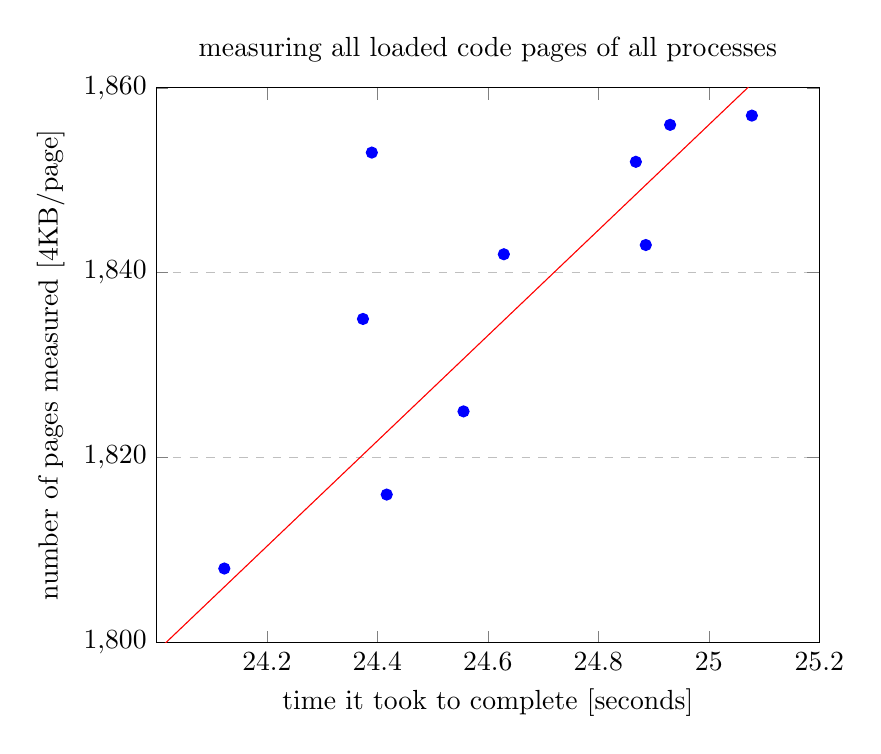
\begin{tikzpicture}
\begin{axis}[
    title={measuring all loaded code pages of all processes},
    xlabel={time it took to complete [seconds]},
    ylabel={number of pages measured [4KB/page]},
    xmin=24, xmax=25.2,
    ymin=1800, ymax=1860,
    xtick={24.2,24.4,24.6,24.8,25,25.2},
    ytick={1800,1820,1840,1860},
    legend pos=north west,
    ymajorgrids=true,
    grid style=dashed,
]

\addplot [
    domain=24:25.2, 
    samples=100, 
    color=red,
]{57*x + 431};

\addplot[
	only marks,
    color=blue,
    mark=*,
    ]
    coordinates {
    (24.868,1852)(24.886,1843)(24.556,1825)(24.930,1856)(24.390,1853)(24.123,1808)(24.417,1816)(24.629,1842)(25.078,1857)(24.374,1835)
    };
    
\end{axis}
\end{tikzpicture}
\caption{Measurement plot for all processes}
\label{graph}
\end{figure}

\paragraph*{}
To provide insight into how long it takes to measure one process (twice), the last experiment was executed on the \textit{init\_proc} process. The results of this experiment can be seen in figure \ref{init}.

\begin{figure}[h!]
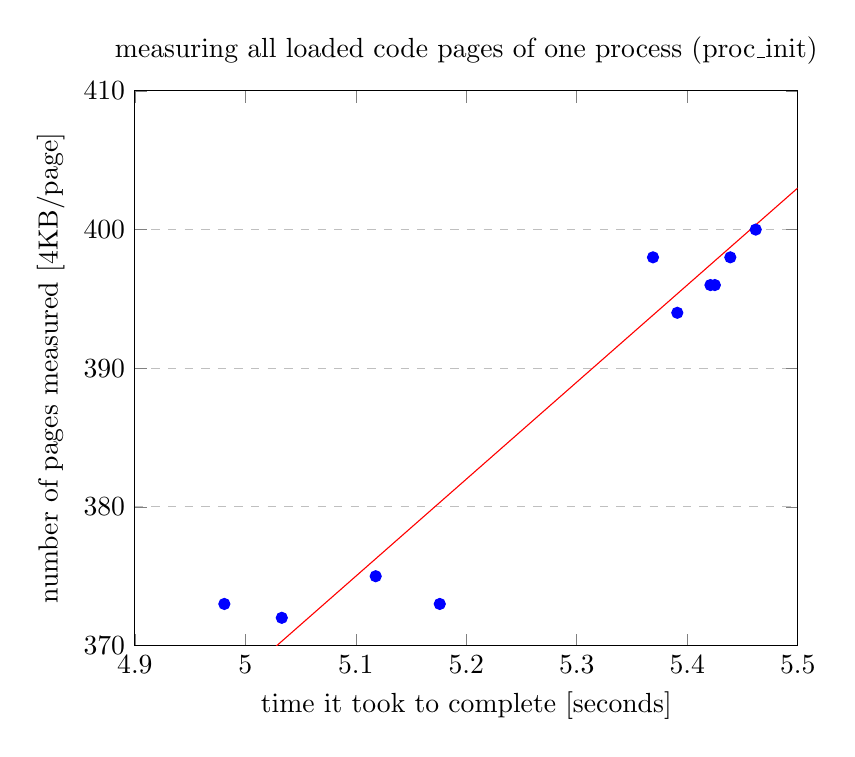
\begin{tikzpicture}
\begin{axis}[
    title={measuring all loaded code pages of one process (proc\_init)},
    xlabel={time it took to complete [seconds]},
    ylabel={number of pages measured [4KB/page]},
    xmin=4.9, xmax=5.5,
    ymin=370, ymax=410,
    xtick={4.9,5,5.1,5.2,5.3,5.4,5.5},
    ytick={370,380,390,400,410},
    legend pos=north west,
    ymajorgrids=true,
    grid style=dashed,
]

\addplot [
    domain=4.9:5.5, 
    samples=100, 
    color=red,
]{70*x + 18};

\addplot[
	only marks,
    color=blue,
    mark=*,
    ]
    coordinates {
    (4.981,373)(5.421,396)(5.369,398)(5.462,400)(5.391,394)(5.033,372)(5.439,398)(5.425,396)(5.118,375)(5.176,373)
    };
    
\end{axis}
\end{tikzpicture}
\caption{Measurement plot for one process}
\label{init}
\end{figure}

\paragraph*{}
In the first two experiments the amount of pages that are loaded into RAM fluctuates a bit. Which probably has to do with pages being swapped in and out of memory. In this last experiment, only one executable memory region of the \textit{init\_proc} is measured and the amount of pages stays constant for all 10 iterations. The amount of pages measured is 88 and the average execution time is 1.319 seconds, the maximum execution time is 1.353, and the minimum 1.299.

\paragraph*{}
Last but not least, the three experiments are plotted in one graph in figure \ref{last} to show how they relate to each other. The mean values of every experiment have been taken to fit each experiment in one data point. They would be very close to one another anyway. This plot clearly shows that the amount of time the measurements take is proportional to the number of pages that are measured. The reason for this is that hashing the memory pages is the most compute-intensive task of the program, and the file overhead is similar, because for every process two files need to be read. This graph allows us to compare the performance of our experiments to that of \cite{LingZhen2021Sbtb}, because we can extrapolate the results to the necessary amount of pages that were measured in the paper. In the paper, 107 MB (of file system image) was measured in 1.276 seconds. We achieve a similar execution time for only 88 executable pages. As explained these were measured twice: once for the initialization phase and once during the attestation phase. This comes down to 352 KB measured twice or 704 KB, which is less than 1\% of their measured memory. If we extrapolate based on the number of pages, it is best to start from the largest experiment to have the least rounding errors. The mean of this first experiment comes down to 1,839 pages measured in 24.625 seconds, 107 MB equals 26 750 pages. Measuring this many pages would require our implementation a little less than 360 seconds or 6 minutes. 

\begin{figure}[h!]
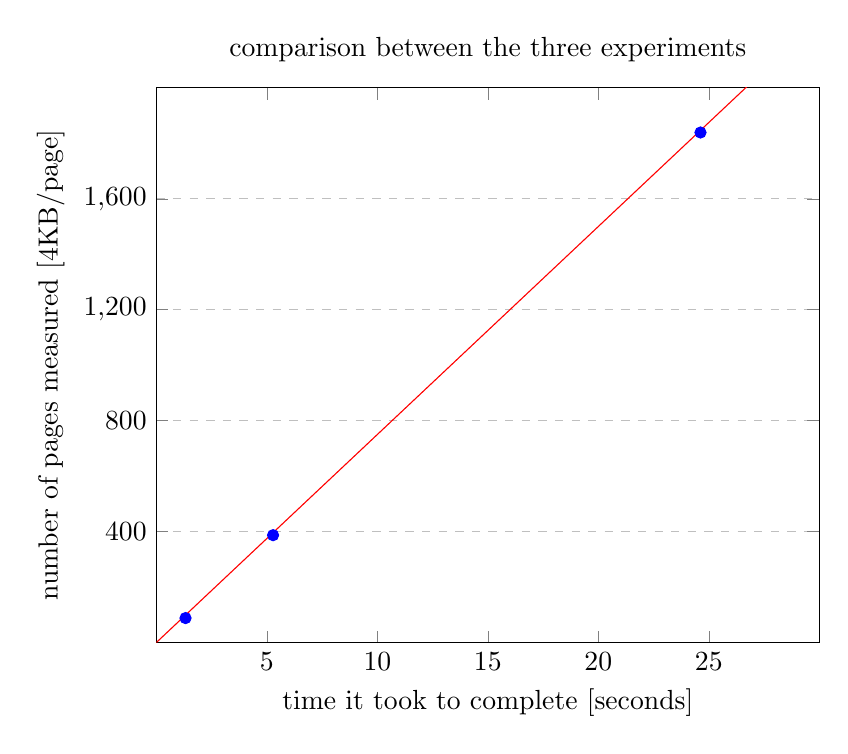
\begin{tikzpicture}
\begin{axis}[
    title={comparison between the three experiments},
    xlabel={time it took to complete [seconds]},
    ylabel={number of pages measured [4KB/page]},
    xmin=0, xmax=30,
    ymin=0, ymax=2000,
    xtick={5,10,15,20,25},
    ytick={400,800,1200,1600},
    legend pos=north west,
    ymajorgrids=true,
    grid style=dashed,
]

\addplot [
    domain=0:30, 
    samples=100, 
    color=red,
]{75*x};

\addplot[
	only marks,
    color=blue,
    mark=*,
    ]
    coordinates {
    (24.625,1839)(5.281,387)(1.319,88)
    };
    
\end{axis}
\end{tikzpicture}
\caption{Comparison of the three measurement experiments}
\label{last}
\end{figure}

\paragraph*{}
As can be seen in the three executed experiments, the performance of the implementation of this work differs a lot from that of \cite{LingZhen2021Sbtb}. Some aspects need some explaining, however. First of all, the implementation is not written nor fine-tuned for performance, it is merely written as a proof of concept. This is due to the memory regions that are attested in this work being only the executable memory pages of a process. These pages need to be identified using multiple files, which generally takes more time compared to the case with one large chunk of memory that is attested. It is also important to take into account that executable pages take up less memory than a file system would generally do. Lastly, these experiments are executed on a Qemu emulation of OP-TEE on a general-purpose laptop (Lenovo Thinkpad P50), while the experiments in \cite{LingZhen2021Sbtb} are executed using a hardware prototype. 

\paragraph*{}
A good balance between performance overhead and security assurance depends on the use case. In the case of a smartphone, we believe even with these results that attesting the executable pages that are loaded in RAM every 30 minutes has not too much impact on the user experience. Depending on the amount of newly loaded memory pages when an application is started, it could even be considered to attest these pages before starting to execute them. This could impact the user experience much more because this happens while the user is waiting for the application to open. While on the other hand, running the attestation in the background on the already loaded pages in RAM, should have minimal impact on the user. These considerations do not take into account the energy consumption of running the attestation, because we didn't have the means for these kinds of experiments.

\section{Security Properties}

\paragraph*{}
The attestation method presented in this work focuses on measuring the code pages of processes loaded in RAM. A code page can only gain control or be executed when it is loaded in RAM first. Keeping this prerequisite in mind, it should suffice to only attest those pages to ensure no corrupted code page gets executed. To put it more mildly, the measurements should run periodically, so a code page may have been executed before the changes are noticed by the attestation PTA.

\paragraph*{}
The integrity of the measurement execution is of utmost importance when it comes to attestation. In RA, the critical code runs on a hardened server, which guarantees that it is infeasible to tamper with the execution control flow. In the case of the PinePhone, the RA method is not used. Instead, user-controlled attestation is applied, which allows the user to verify the trustworthiness of his device. The critical code which compares the measurements runs in the SW. The TEE provided by ARM TrustZone does guarantee that the NW cannot influence the execution of the SW in any way, as long as the device was started up successfully using secure boot.

\paragraph*{}
Secure storage of results is very important for a liable attestation method. If an adversary were able to tamper with these values, they could make every attestation attempt fail due to the changed initial value. In case a bad hashing algorithm is chosen and the attacker can read the initial hash digest, he could also try to forge a collision attack \cite{SafaryanOlga2021MHCC} where he tampers with a page in such a way that its hash digest does not change but the code in the page does something the attacker desires. To make sure the reference values are not tampered with, they need to be stored in secure memory which should not be accessible from outside the SW. In the SW, these values should only be written during the initialization phase and afterward only read. This needs to be stated less strictly. In case there are software updates or additional software to be installed on the device, the initial values will have to be overwritten. The initialization phase could be executed again to update or add the measurement results for those code pages. 

\section{Security Evaluation}

\paragraph*{}
Security guarantees that can be made, are the integrity of the measurement execution control flow and the integrity and confidentiality of the results that are being stored. These are achieved thanks to secure boot process enabling the TEE of ARM TrustZone. These are key assumptions in the field of RA, and thus are also very important in this case of user-controlled attestation. Of course, when discussing the security guarantees of a certain solution, it is not only about the execution and storage of the measuring application itself, but also about what additional security guarantees it provides to the system overall. The most important guarantee that an attestation solution tries to provide, is being able to detect modifications or unexpected possibly malicious changes to the aspects of the system it attests. In our case, the code pages of processes are being attested, we only measure the ones that are present in RAM, because only then they are able to harm the system. As stated in \cite{LingZhen2021Sbtb} there is still an unsolved problem, the rich OS needs to provide the physical addresses of the code pages. This means that malware capable of self hiding or transient rootkits are still possible threats that could stay unnoticed by this solution. If an adversary has taken control of the OS, there are countless ways in which the attacker could deny the attestation PTA to obtain the necessary addresses, which would be very hard to identify and alert the user.

\paragraph*{}
OS/firmware attacks are present in the attacker model of \cite{LingZhen2021Sbtb} on which this work is based. We believe that with this method the code pages of all processes, including those of the rich OS, can be attested and this will enable the user to be notified about any tampering with this code base. This does not mean, however, that tampering with these code pages has become harder. Besides tampering with code, there are also lots of different methods to perform an OS/firmware attack. We believe that this work can be extended to thoroughly attest the NW, but in its current state it only allows detection of a small portion of the OS/firmware attack surface.

\paragraph*{}
It is also claimed by \cite{LingZhen2021Sbtb} that software attacks are protected against or detectable in the case of attestation. Again, with their addendum about only securing the code section of processes, this is valid but the integrity of the code is only a small portion of the attack surface. In their measurement method, the data structures are not checked, and those are the main target for very well-known attacks that have been around for decades, like buffer overflows and return-oriented programming. Extensions to this solution need to be realized to detect software attacks, OS/firmware attacks likewise.
\chapter{Discussion}

\section{Related work}

\paragraph*{}
The paper on RA, secure and trusted boot on IoT Nodes \cite{LingZhen2021Sbtb} is the paper on which the implementation and experiments of this thesis are based, and is extensively explained in the background section. To provide a better understanding of the effectiveness of their solution, it is compared to three related works. Preceding this comparison, these three papers are briefly explained with in depth explanations on the parts that are most relevant for the comparison. The main focus of this comparison will be on the added security guarantees and the assumptions that have been made with respect to the RA. After the comparisons of the related work, the weaknesses and possible improvements of the work performed in this thesis will be discussed.

\subsection*{SecTEE: A Software-based Approach to Secure Enclave Architecture Using TEE}

\paragraph*{}
The solution described in the paper about SecTEE \cite{ZhaoShijun2019SASA} aims to implement a framework using ARM TrustZone to achieve similar security guarantees as a hardware-based secure enclave architecture. The authors provide the following contributions with their paper. Their first contribution is the implementation of SecTEE, the new secure enclave architecture which achieves \textit{\enquote{the highest level of security}} using ARM TrustZone. Secondly, a locking mechanism is introduced which makes sure enclave pages cannot be accessed while the enclave is running to prevent cross-core side-channel attacks. The TEE OS is also extended to provide functionality like identification, RA, and sealing sensitive data. Lastly, an implementation of SecTEE based on OP-TEE is provided along with experiments showing the performance of the proposed system. 

\paragraph*{}
Their wording of \textit{\enquote{the highest level of security}} means that it should be resistant to privileged host software attacks, board-level physical attacks, page fault based side-channel attacks, and cache based side-channel attacks. The hardware attacks on which is focused are cold boot attacks \cite{HuberManuel2016Afff}, bus monitoring attacks \cite{TPMGenie}, and Direct Memory Access (DMA) attacks. Attacks against the internal state of the SoC are not considered, because those are assumed to be very sophisticated and require expensive equipment. To achieve this security, certain requirements are necessary. First of all, a Device Sealing Key (DSK) needs to be present. This is a symmetric key only known by the device itself and used to protect secrets related to the device. Also needed is a Device Root Key (DRK), which is an asymmetric key pair necessary to identify and authenticate the device. Lastly, the manufacturer's public key needs to be hard coded on the device to make sure it is able to verify the signature on software updates from the manufacturer. 

\paragraph*{}
An important aspect of the SecTEE architecture is the method that is applied for memory protection. SecTEE protects enclaves from physical attacks by using a similar approach as the OP-TEE pager. It is an on-demand paging system which runs the entire TEE system on OCM. Whenever a page leaves this OCM, it is encrypted to ensure confidentiality and integrity of the data while it is stored on the Dynamic Random Access Memory (DRAM). Another key feature of SecTEE is its side-channel resistance. Side-channel attacks from the SW are avoided by using a page coloring mechanism. Different enclaves can never share the same cache set, which ensures that one enclave will never be able to evict cache lines of another one. Of course, side-channel attacks can also come from the NW, especially because the NW and SW share the same cache in the ARM TrustZone architecture. In the NW, there are of course certain limitations to what is possible with the cache lines due to privilege restrictions. Nonetheless, the prime and probe method is still relevant in this case. SecTEE cleans and invalidates all cache levels when the Central Processing Unit (CPU) switches from the SW to the NW. This, however, is not sufficient because cross-core side-channel attacks can launch the attack, while a core of the CPU is still executing in the SW. To handle this problem, the cache set of the enclave is locked, which guarantees that the cache of the enclave cannot be probed or manipulated by the NW. Some final aspects that deserve some highlighting are enclave identification, measurement, and RA in SecTEE. Enclaves are published along with the public key of the author and the signed integrity value of the image. With this information the enclave can be verified and identified before it is run. During runtime, the enclave keeps track of important aspects like enclave identifier, integrity, and a flag indicating whether it is privileged. For the RA a specific quoting enclave is created. This is a privileged enclave that can make the system calls related to the management of attestation keys, other enclaves are not allowed to do this. These keys are used to sign the report data of the attestation together with the runtime measurement to provide proof to the verifier that it comes from the correct enclave.

\paragraph*{}
First of all, the number of lines of code are measured because these implementations extend the TEE kernel. This is the TCB and needs to be kept minimal because bugs could easily introduce security vulnerabilities. Next, the overhead of the trusted computing features is identified and discussed. This overhead is acceptable in case Elliptic Curve Cryptography (ECC) with keys of 256 bits are used, some system calls take too long in case Rivest-Shamir-Adleman (RSA) keys of 2,048 bits are used. The performance of certain enclaves was measured and the xtest benchmark of OP-TEE was executed. SecTEE was about 4 times slower than OP-TEE on the benchmark and 40 times slower than OP-TEE on the enclave execution. It is argued that the memory protection mechanism is the cause of the greatest performance overhead in SecTEE. Finally, to test the effectiveness of the side-channel defense, the effectiveness of the attack on plain OP-TEE is compared to the case of SecTEE. In case of a NW attack, there is a clear difference between prime and probe timings in OP-TEE while both memory operations take an equal amount of time when using SecTEE. This makes it impossible for an attacker to learn anything about the cache behavior of the victim enclave in SecTEE. For the SW attack an Advanced Encryption Standard (AES) key could be recovered after 256,000 encryptions in OP-TEE, while in SecTEE the attacker could not learn any information about the used key.

\subsection*{TrustShadow: Secure Execution of Unmodified Applications with ARM TrustZone}

\paragraph*{}
TrustShadow \cite{GuanLe2017TSEo} is designed to protect existing applications from untrusted OSs without the need to modify the applications themselves. This is achieved by using TrustShadow as a lightweight runtime system that shields the sensitive information of the application from the OS. This system does not provide system services itself but requests them from the OS. It does, however, guarantee security through encryption, context switching and verifying return values. To ensure that the OS cannot get hold of the encryption keys, sensitive data, and cannot interfere with the security verification, TrustShadow runs in the SW of the ARM TrustZone processor.

\paragraph*{}
The solution described in the paper about TrustShadow is mainly focused on protecting applications from an untrusted OS. This means that the attacker is able to launch DMA attacks, modify interrupted process states, change program execution control flow, hijack system services, and control communication channels \cite{QiangChenyi2018CCAD}. DoS attacks and side-channel attacks such as timing and power analysis are not taken into account in this solution.

\paragraph*{}
The memory of the different stakeholders is isolated from each other to make sure the rich OS is not able to tamper with the memory of the applications and with the runtime system. TrustShadow utilizes the TZASC to make three partitions in memory: one unprotected for the applications, one protected for the applications and one protected for the runtime system itself. The virtual memory space is equally distributed between the OS and the runtime system TrustShadow. The runtime system also maps the physical address space holding the OS to efficiently locate shared memory. Another aspect that needs to be taken into account, is that the OS is used to handle exceptions. When an exception is thrown, the state of the application is stored and the state of the OS is restored. The runtime system then reproduces the exception in this OS state to allow the OS to handle it without the need to get sensitive details about the application. There are two exceptions that the runtime system implemented in the SW, namely, the random number generation, and floating point operations. Since the cryptography relies on the security of these exceptions they are security critical. System calls are similar to exceptions: the OS needs some information about the application requesting the system call. TrustShadow sanitizes this information to make sure only the necessary data is received by the OS. After receiving the result from the system call, the runtime system also checks this result on correctness before forwarding it to the application. An example of sensitive information that an untrusted OS should not have access to is the memory mapping from virtual to physical address space. This information is stored in the page tables. TrustShadow makes use of the OS page fault handler to update and retrieve the page table entries that are stored in the SW. This ensures that the rich OS does not require the information because it is controlled by the runtime system. After the memory location of a page has been found, this can be loaded for execution. Before this loading is finished, however, the page is checked on its integrity. TrustShadow verifies the executable pages of an application and the executable pages of the shared libraries based on a manifest file related to the application. 

\paragraph*{}
TrustShadow was evaluated with a variety of measuring methods. Microbenchmarks using LMBench, file operations using Sysbench, HTTP and HTTPS request handling using Nginx, and finally, the performance overhead on data analytic applications. The performance overhead caused by the runtime system was negligible across all tests. In terms of security, the OS still has a lot of control: it could, for instance, invoke a system call with the original \textit{execve} instead of the new \textit{tz\_execve} which largely bypasses TrustShadow. Another concern is the possibility to manipulate or forge manifest files which could allow an attacker to tamper with the code of an application without the runtime system being able to detect it. 

\subsection*{TZ-MRAS: A Remote Attestation Scheme for the Mobile Terminal Based on ARM TrustZone}  

\paragraph*{}
In this paper \cite{WangZiwang2020TARA}, a TrustZone based Mobile Remote Attestation Scheme (TZ-MRAS) is proposed. There are three main challenges the authors tackle, the first one is building a RoT for measuring, storage, and reporting of the attestation results. The second challenge is to execute binary-based attestation on hardware constrained devices while defending against TOC-TOU attacks. The last challenge consists of the performance optimization of storing measurement logs in a hash tree which has considerable overhead during the construction and updating phases. 

\paragraph*{}
The assumptions of the TrustZone model are followed, meaning that the processor is trusted and a CoT is achieved to trusted applications. The SW is the TCB and it provides features to attest the integrity of the NW. The attacker, on the other hand, is assumed to have kernel level access, meaning he can tamper with the REE kernel and applications in any way he desires. DoS and side-channel attacks are not considered in this paper.

\paragraph*{}
To tackle the first challenge related to the root of trust, the functionality of a TPM chip is provided by the TEE of TrustZone. These functionalities are implemented in TA's running in the SW to ensure isolation from the NW. The measurement module keeps track of REE and dynamically detects integrity changes in the kernel, but can also update the Secure Measurement Log (SML). Secondly, the TOC-TOU attacks are protected against by updating the SML with a dynamic update mechanism, namely ProbeIMA. Probes are added to all operations that are able to modify the code pages of the kernel, meaning that any attempt to execute any of these operations will be detected. Lastly, the structure of the SML is optimized by storing the root node in a hardware protected register and the rest of the hash tree in secure memory. Also, the design related to the construction, insertion and revocation algorithms avoids too frequent construction and update operations to increase performance.

\paragraph*{}
The performance overhead in terms of execution time difference, is only touched on shortly. Because this is less than 10\% in the worst case, which is very acceptable. Besides the performance overhead, the security analysis is backed up with experiments that show the solution works, and is able to detect the attacks used. The simulated attacks are a rootkit that hijacks the kernel function of the system call table and a TOC-TOU attack that modifies the code pages, and restores them again in between integrity checks. Lastly, the depth of the hash tree is measured for a varying amount of updated nodes, mainly to prove that the construction and updates on those trees have a limited impact on performance.

\section{Comparison of Approaches}

\subsection*{Effectiveness}

\paragraph*{}
All solutions focus on measuring the binaries of the executable files to verify the integrity of the runtime system. This is achieved by having a TA in the SW which does the measurements, stores the results, and encrypts them before sending them to the RA server. Running the attestation inside the SW shields the attestation process from being tampered with by the NW. But it does not guarantee that the execution control flow of the attested applications cannot be tampered with. SecTEE seems to keep track of more data for the attestation process, but nothing is said about the integrity of data structures or other critical parts of the system. 

\paragraph*{}
Except for the paper on SecTEE, all solutions have a very similar goal and their solutions are also very comparable. All three solutions (TrustShadow, TZ-MRAS and the trusted boot) mainly focus on the attestation of NW processes, but these are not very well shielded or isolated from the rich OS. SecTEE uses RA as one of the many tools to protect the applications or at least identify violations thereof. Due to the effort the authors of SecTEE put into the memory protection scheme, the page coloring mechanism and the way enclaves need to be implemented, it achieves better security guarantees for the enclaves. An enclave has to be implemented as a TA, which by itself introduces additional security guarantees like, it being infeasible for the rich OS to tamper with the execution control flow of the enclave.

\paragraph*{}
None of the solutions mentioned give much attention to the openness of the secured system. SecTEE, for instance, requires a private public key pair from the manufacturer to function, which entirely closes the solution towards the user and third parties that may also provide useful software. The DRK used in that architecture could serve as the RoT of the device. The other examples do not explicitly mention how the RoT is achieved, only that it is stored in tamper resistant storage hardware. This is, however, a very important detail when validating the openness of the final system.

\subsection*{Assumptions}

\paragraph*{}
All solutions assume an IoT device or smartphone device meaning, the solutions need to be adapted to devices with limited hardware specifications. Based on this assumption, all compared solutions chose for ARM SoC with TrustZone capabilities. In this context the SW of ARM TrustZone, along with its TAs, are all assumed to be trusted and secure and isolated from the rich OS. In the case of SecTEE, the additional assumption is made that the enclaves (isolated applications) are written as TAs, which may be feasible for an open platform. Although when these enclaves need to be signed by a manufacturer's private key, it achieves an entirely different goal. On the other hand, the other solutions claim to attest the NW and provide similar protection against the rich OS, which is unfeasible if only the code pages of an application are measured for integrity violations. 

\paragraph*{}
SecTEE claims to protect against certain side-channel attacks and hardware attacks like DMA and cold boot attack. These claims seem to be met thanks to the SW being instantiated in a trusted manner with secure boot and the protected code running in the SW. The papers about TrustShadow and TZ-MRAS acknowledge that side-channel attacks are not dealt with, but DMA attacks are prevented by protecting the address space mapping and encrypting the stored data. The reproduced solution does not give specific details about side-channel attacks or DMA attacks, it only mentions hardware, software, and OS attacks. These claims seem excessive, because only the attestation TA itself is protected against these kinds of attacks, due to the TEE and trusted boot. The applications in the NW are still vulnerable to many attacks of which only a few (changing the executable code of the application) are detected by the solution. Last but not least, OS attacks cannot be prevented using this method. An attack can in some cases (depending on what is modified) be detected with RA, but none of the solutions make an effort to make attacking the OS harder. This is due to it not being considered when discussing the applications running in the NW.

\section{Reflection}

\paragraph*{}
First of all, a consideration needs to be made with respect to the RoT of the system. The discussed related work does not take into account the openness of the system, and thus does not discuss this in detail. The PinePhone is equipped with tamper resistant storage hardware, which could accommodate the RoT. This detail on what exactly is stored in this memory and how this information is generated, has a large impact on whether the system remains open. If the user is allowed to put a public key in the secure storage, of which he and only he possesses the secure counterpart, the solution remains open. The security, of course, depends on how well the user is able to protect his private key, but this is out of scope for this work. This is, however, how we believe a RoT can be achieved for an open system. In case the device is sold second-hand, there is of course a problem, because the buyer needs to trust the first owner in order for this deal to work. Since the original user possesses the private key, and it is hard to prove that when the buyer receives this key, the initial owner does not have access to this key anymore. This is interesting, but goes beyond realizing a secure RoT for an open platform.

\paragraph*{}
Our solution avoids the trusted third party that needs to be convinced that the integrity of the software running on the device is not violated. The only party that needs to be assured about the integrity of the system is the user. Based on our implementation we can claim that the NW process integrity checking works. To become a complete security solution, certain extensions will need to be made which are discussed in the future work. Taking these considerations into account, we believe that user-controlled attestation can be used to increase the security of an open platform without disrupting the openness of the system.

\paragraph*{}
The evaluation gives insight in how well this solution meets the expectations of the smartphone user. The performance is not ideal as elaborately discussed earlier, but this was not the main goal of the proof of concept. Making sure the solution meets the expectations of the user is one thing, but the software providers need to be confident about their guarantees as well. Right now the user decides which software can run on the device. By doing so he is assumed to trust the software provider. A software provider is only guaranteed that, other software running on the platform comes from providers that are trusted by the user. This guarantee is not very strong, since there is a possibility that the user trusts a malicious provider which could try to tamper with the processes of other providers. If software providers need additional guarantees, the attestation solution should be extended to provide these security measures, some examples of these measures are given in the future work. Even though guaranteeing the software providers correct execution control flow of their processes seems evident, it does have implications on the user's freedom to operate the device. This leans more towards the philosophical side of the open platform idea so we will not dive in too deep about this.

\paragraph*{}
The solution in this thesis differs from \cite{LingZhen2021Sbtb}, in the sense that the initial measurement results are stored in the secure memory of the SW instead of at a RA server. Storing these values on the device itself, allows for the solution to be extended, and allow the user to attest the device. Depending on how the user reacts to this information, similar security guarantees can be provided as the closed systems. All related work that we have discussed, relies on the integrity and confidentiality of the secure memory of ARM TrustZone. Furthermore, the execution control flow of the TAs is always assumed to be protected against adversaries whether they attack with software attacks, OS attacks, or certain hardware attacks. The solution presented in the implementation also relies on these features to store the initial hash digests and perform the comparisons with the newly measured values, respectively. Due to these assumptions already being present they do not weaken the security of the proposed system compared to the closed systems.

\section{Future Work}

\subsection*{Considerations}

\paragraph*{}
One important sensitivity point is to decide whether every page in an executable memory region gets its own hash value or whether all the pages in this memory region get one combined hash value. The fine-grained option allows to only measure the code pages that are currently loaded into the RAM. This is sufficient, because the executable page can only start being executed when it is located in RAM. If, on the other hand, all pages of the region need to be measured, the unused pages also need to be loaded into RAM to be able to measure them. The downside to the fine-grained option is that more initial values need to be stored, since every page has its own value.

\paragraph*{}
Another trade-off that could be put forth, is the hashing algorithm that is used to measure the memory pages. The hashing algorithm needs to adhere to certain requirements like avoiding collisions, but a Hash-based Message Authentication Code (HMAC) algorithm that uses a key during the hashing process, is definitely excessive. The hashing mainly needs to be fast, because lots of memory pages need to be attested and this needs to happen relatively often to guarantee improved security. The hash digests do not need to be secure in the sense of being unforgeable. They are stored in secure memory which cannot be tampered with, meaning the attacker is not able to replace the initial values with a malicious one. With the initial values assumed secure, the hash digests are merely used to detect whether the hashed information has changed or not, for which a normal hashing algorithm is sufficient due to its collision avoidance.

\paragraph*{}
Lastly, it was found out that in a recent framework update of OP-TEE an attestation PTA was added to the kernel \cite{OPTEE3.17}. The PTA in that solution attests the SW processes (TAs), which is different from the implementation presented in this thesis, since we focus on checking the integrity of the processes in the NW. This also implies that the added PTA in the kernel provides asymmetric key encryption to communicate with a remote verifier in a secure manner. The update notes clearly state that RA was intended, so these differences are definitely in line with the expectations. Even though there are certain differences, it is definitely possible to change the implementation 'slightly' to make it fit into this provided attestation PTA and reuse some of its already present functionality. This could be the beginning of a more standardized form of NW integrity checks if the shortcomings have been dealt with.

\subsection*{Shortcomings}

\paragraph*{}
In the proposed solution, there is still a strong dependency upon the rich OS. This dependency mainly comes from the files that are used to determine the physical addresses of pages related to the processes that are measured. These files are part of the data structures the rich OS owns. A solution to this problem could be to move the responsibility of the memory mapping into the SW. The downside to this is that it increases the TCB, because the SW is often seen as the TCB. This can however be achieved in a relatively lightweight fashion, as demonstrated in the TrustShadow paper where the page table is stored inside the SW, and the SW handles page faults that are generated in the rich OS. 

\paragraph*{}
Partial attestation introduces a fake sense of security, because not all possible attacks are checked. We have mentioned that the execution control flow of an application can be tampered with through the manipulation of data structures. There are lots of ways similar attacks can be achieved to make applications behave differently than intended. Some solutions protect better against some of these attacks than others, like checking the results of a system call executed by the rich (untrusted) OS. \cite{MuhlbergJanTobias2016LaFT} describes a variety of possible aspects for which integrity checks are useful to increase the level of trust one can have in an application. These properties vary from OS data structures, available resources to event occurrence and timing. This is probably harder to achieve when trying to protect against a rich OS like Linux compared to the Contiki OS that was used, but it looks like a promising direction for future work.

\paragraph*{}
The attestation measurements are performed, software integrity checks in our case, but there is no way to interact with this information yet. To allow the user to perform user-controlled attestation, he needs to be informed about the results of these measurements. To make sure this is achieved in a secure manner, the trusted I/O channels in ARM TrustZone can be used. Through these channels the user could also command the system to take certain actions with respect to the processes that have been tampered with. By doing this the user is in control with respect to how software integrity violations are handled.

\paragraph*{}
Finally, if software providers need to be guaranteed that the execution control flow of their programs is not tampered with, an extension is necessary. For instance, the ability to identify applications violating security measures like trying to tamper with other applications or the rich OS. The user should be notified about this and be strongly advised to remove those malicious applications from his device. A solution could be opted for where the process is terminated if any inconsistencies are detected. This would increase the guarantees that can be provided with respect to the proper execution of programs from certain software providers. It would of course be better if it were infeasible to tamper with another process, but we believe this is not achievable with user-controlled attestation or any form of attestation alone.
\documentclass{report}

\raggedright

\begin{document}

\chapter{Conclusion}

To achieve secure execution on the PinePhone some requirements need to be met. One of these requirements is that a chain of trust is achieved which is done using secure boot in this case.

\section{Related work}

\begin{itemize}
\item Secure boot, Trusted boot and remote attestation for ARM TrustZone-based IoT Nodes
\item DAA-TZ: An Efficient DAA Scheme for Mobile Devices Using ARM TrustZone
\item SecTEE: A Software-based Approach to Secure Enclave Architecture Using TEE
\item TZ-MRAS: A Remote Attestation Scheme for the Mobile Terminal Based on ARM TrustZone
\item TrustShadow: Secure Execution of Unmodified Applications with ARM TrustZone
\end{itemize}

\section{Comparison of Approaches}

\begin{itemize}
\item Effectiveness \begin{itemize}
\item Reached goal
\item Defends most variety of attacks
\item Stronges security guarantees
\end{itemize}
\item Assumptions \begin{itemize}
\item Least assumptions
\item Most realistic
\end{itemize}
\end{itemize}

\section{Future Improvements}

\begin{itemize}
\item Best approach \begin{itemize}
\item Overview
\item Reasoning
\end{itemize}
\item Weaknesses
\item Possible improvements \begin{itemize}
\item inspiration from Lightweight and Flexible Trust Assessment Modules for the Internet of Things
\end{itemize}
\item Different solutions
\end{itemize}

To allow the user to attest their device it is important that Trusted I/O is used to inform the user about the outcome of the attestation process.
\medskip

The attestation application can be seen as one module that can be accompanied with a variety of different modules to increase the amount of checks that can be executed to check more possible attacks/ vulnerabilities.

\end{document}


% If you have appendices:
%\appendixpage*          % if wanted
%\appendix
%\chapter{The First Appendix}
\label{app:A}
Appendices hold useful data which is not essential to understand the work
done in the master's thesis. An example is a (program) source.
An appendix can also have sections as well as figures and references\cite{h2g2}.

\section{More Lorem}
\lipsum[50]

\subsection{Lorem 15--17}
\lipsum[15-17]

\subsection{Lorem 18--19}
\lipsum[18-19]

\section{Lorem 51}
\lipsum[51]

%%% Local Variables: 
%%% mode: latex
%%% TeX-master: "thesis"
%%% End: 



\backmatter
% The bibliography comes after the appendices.
% You can replace the standard "abbrv" bibliography style by another one.
\bibliographystyle{ieeetr}
\bibliography{references}

\end{document}

%%% Local Variables: 
%%% mode: latex
%%% TeX-master: t
%%% End: 
